\begin{frame}[containsverbatim]
	\frametitle{Example: One-way MANOVA-- Romano-British Pottery}

  \begin{itemize}
  	\item Tubb, Parker \& Nicholson used atomic absorption spectroscopy
	to analyze the chemical composition of 26 samples of Romano-British
	pottery found at four kiln sites in Britain.
	\begin{itemize*}
		\item \alert{Sites}: Ashley Rails, Caldicot, Isle of Thorns, Llanedryn
		\item \alert{Variables}: aluminum (Al), iron (Fe), magnesium (Mg),
	calcium (Ca) and sodium (Na)
		\item $\rightarrow$ One-way MANOVA design, 4 groups, 5 responses
	\end{itemize*}
	
	\item Can the content of Al, Fe, Mg, Ca and Na be used to 
	differentiate the sites?
  \end{itemize}

\begin{CodeInput}
R> library(heplots)
R> pottery.mod <- lm(cbind(Al, Fe, Mg, Ca, Na) ~ Site, 
                     data=Pottery)
R> Manova(pottery.mod)
\end{CodeInput}
\begin{CodeOutput}
Type II MANOVA Tests: Pillai test statistic
     Df test stat approx F num Df den Df    Pr(>F)    
Site  3    1.5539   4.2984     15     60 2.413e-05 ***
---
Signif. codes:  0 '***' 0.001 '**' 0.01 '*' 0.05 '.' 0.1 ' ' 1 
\end{CodeOutput} 
\end{frame}

\begin{frame}
	\frametitle{HE plot details: Scaling \H and \E}

  \begin{columns}[T]
    \begin{column}{.6\textwidth}
	  \begin{itemize}
  		\item<1-> The E ellipse is divided by $df_e = (n-p) \rightarrow$ data ellipse of
		residuals
			\begin{itemize*}
			\item<1-> Centered at grand means $\rightarrow$ show factor means in same plot.
			\end{itemize*}
		\item<1-> ``Effect size'' scaling-- $\H / df_e$ $\rightarrow$
		data ellipse of fitted values.
		\item<2-> ``Significance'' scaling-- H ellipse protrudes beyond
		E ellipse \emph{iff} $H_0$ can be rejected by Roy maximum root test
			\begin{itemize*}
			\item $H / ( \lambda_\alpha df_e )$ where $\lambda_\alpha$
			is critical value of Roy's statistic at level $\alpha$.
			\item direction of \H wrt \E \implies linear combinations that
			depart from $H_0$.
			\end{itemize*}
	  \end{itemize}
    \end{column}
    \begin{column}{.4\textwidth}
    \includegraphics<1>[width=\textwidth,clip]{fig/pottery2-1}
    \includegraphics<2>[width=\textwidth,clip]{fig/pottery2-2}
    \end{column}
  \end{columns}
\vspace{1em}  
\only<1>{
%\begin{CodeInput}
%R> heplot(pottery.mod, size="effect")
%\end{CodeInput}
\hfill\red{\textbf{\texttt{R> heplot(pottery.mod, size="effect")}}}
}	
\only<2>{
\hfill\red{\textbf{\texttt{R> heplot(pottery.mod, size="evidence")}}}
}	
\end{frame}

\begin{frame}
	\frametitle{HE plot details: Contrasts and linear hypotheses}
  \begin{columns}[T]
    \begin{column}{.6\textwidth}
	  \begin{itemize}
	    \item<1-> An overall effect \implies an \H ellipsoid of
		$s = \min( p, df_h)$ dimensions
		\item<2-> Linear hypotheses, of the form 
		$H_0 : \mat{C}_{h \times q} \, \vec{B}_{q \times p} = \mat{0}_{h \times p}$
		\implies sub-ellipsoid of dimension $h$
		\item<3-> 1D tests and contrasts \implies degenerate 1D ellipses (lines)
	  \end{itemize}
    \end{column}
    \begin{column}{.4\textwidth}
    \includegraphics<1>[width=\textwidth,clip]{fig/pottery1-1}
    \includegraphics<2>[width=\textwidth,clip]{fig/pottery1-2}
    \includegraphics<3>[width=\textwidth,clip]{fig/pottery1-3}
    \end{column}
  \end{columns}

%% \begin{block}<2->{Conjecture}
 Every linear hypothesis of $h$ degrees of freedom nested within an $s$ degrees of freedom
 larger test corresponds to a sub-ellipsoid of dimension $h$ touching the dim($s$) at
 exactly two points.
%% \end{block}
\end{frame}

\begin{frame}
	\frametitle{HE plot matrices: All bivariate views}
	\begin{center}
      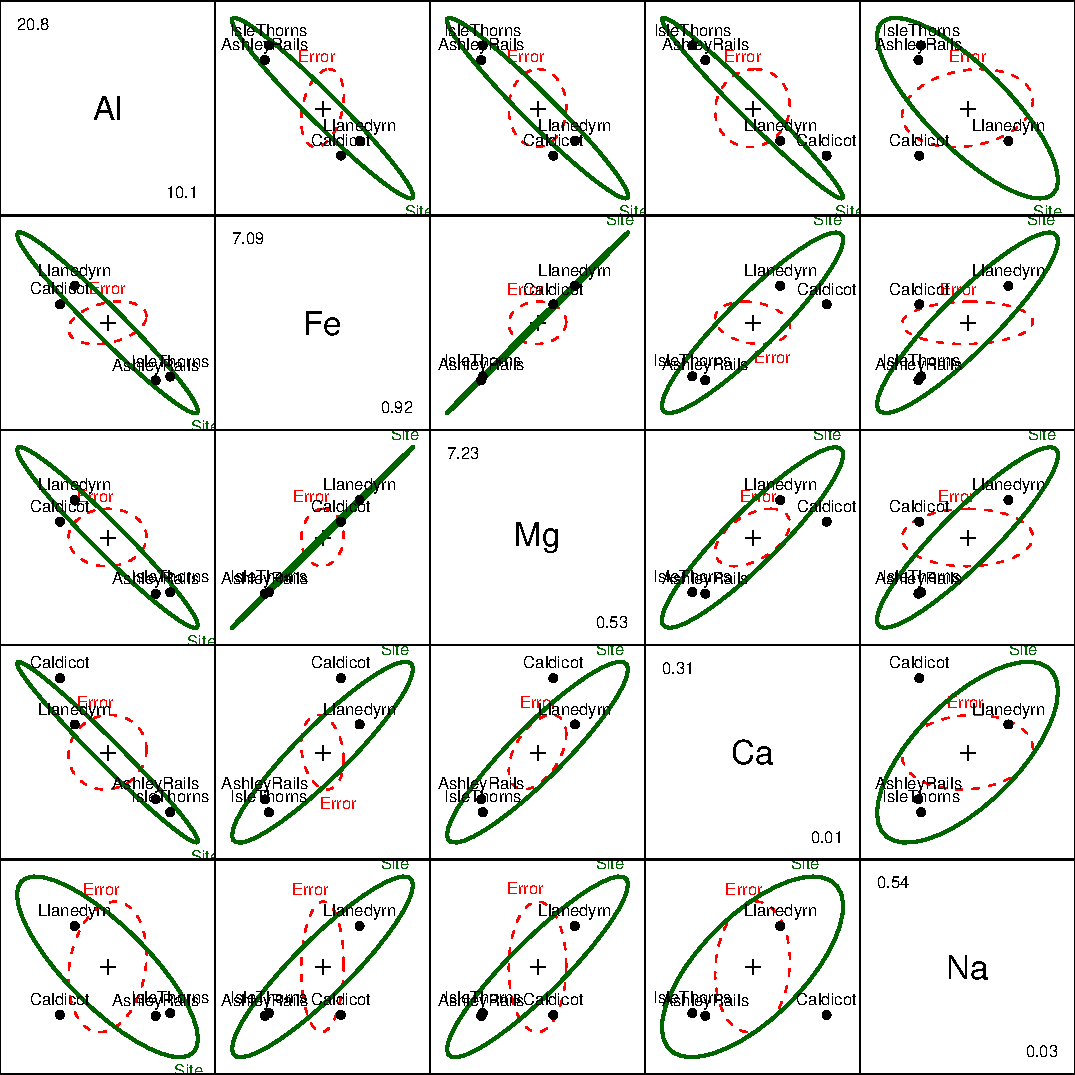
\includegraphics[height=.8\textheight,clip]{fig/pottery3-1}
	  \\
	  \red{\textbf{\texttt{R> pairs(pottery.mod)}}}
	\end{center}
\end{frame}
